% F091｜verify 原创简明教学示意图
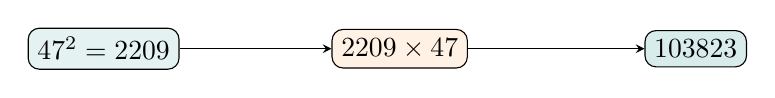
\begin{tikzpicture}[>=stealth,scale=.94]
\node[draw,fill=teal!10,rounded corners] (a) at (0,0){$47^2=2209$};
\node[draw,fill=orange!10,rounded corners] (b) at (4,0){$2209\times47$};
\node[draw,fill=teal!15,rounded corners] (c) at (8,0){$103823$};
\draw[->] (a)--(b);\draw[->] (b)--(c);
\end{tikzpicture}
